\subsection{Caso d'Uso: Controproposta di un'Offerta}

Il caso d’uso Controproposta di un’offerta è stato progettato seguendo la stessa logica di interazione non intrusiva adottata per altre operazioni simili.
L’obiettivo principale è mantenere la continuità del contesto visivo, riducendo al minimo le interruzioni nel flusso di lavoro dell’utente. Per questo motivo, l’azione viene gestita all’interno di una finestra modale (popup) che consente di operare senza abbandonare la vista principale.

\vspace{0.5cm}
\subsubsection{Struttura e Flusso dell’Interazione}
L’interazione si articola in più fasi distinte, ognuna delle quali mira a garantire chiarezza e controllo all’utente:
\begin{itemize}
	\item \textbf{Popup iniziale}: la finestra modale mostra i dettagli della proposta selezionata (mittente, testo sintetico e valore corrente) e include un campo dedicato all’inserimento del nuovo valore della controproposta.
	In calce è presente un pulsante di azione principale con etichetta \textbf{«Invia controproposta»}.
	
	\item \textbf{Conferma dell’invio}: al clic su \textbf{«Invia controproposta»}, viene visualizzato un dialog di conferma per prevenire invii accidentali.  
	I pulsanti di conferma e annullamento sono caratterizzati da colori neutri, così da differenziarli visivamente dalle azioni primarie della piattaforma e migliorare la leggibilità percettiva \cite{nielsen1995}.
	
	\item \textbf{Feedback di caricamento}: dopo la conferma, il sistema mostra una barra di avanzamento stilizzata con i colori istituzionali dell’applicazione.  
	Anche in presenza di tempi di risposta brevi, viene introdotto un lieve ritardo percettivo per garantire un feedback visivo chiaro sull’elaborazione in corso \cite{shneiderman2004}.
	
	
\end{itemize}

\vspace{0.5cm}
\subsubsection{Esito dell’Operazione e Aggiornamento della Lista}
Al completamento dell’operazione, il sistema applica una serie di aggiornamenti automatici per riflettere lo stato corrente:
\begin{itemize}
	\item la finestra modale viene chiusa automaticamente;
	\item nella lista delle proposte, la voce corrispondente viene aggiornata con il nuovo valore della controproposta;
	\item il testo della proposta precedente può essere troncato o sintetizzato per preservare la leggibilità complessiva della tabella;
	\item lo stato della proposta viene aggiornato a \emph{«Controproposta inviata»}, rendendo immediatamente visibile l’esito dell’azione.
\end{itemize}

\vspace{0.5cm}
\subsubsection{Considerazioni di Usabilità e Sicurezza}
La soluzione basata su finestra modale garantisce un’esperienza utente coerente con i principi di usabilità e sicurezza dell’interfaccia:
\begin{itemize}
	\item \textbf{Continuità contestuale}: l’utente rimane all’interno del proprio flusso operativo, con possibilità di annullamento rapido.
	\item \textbf{Prevenzione degli errori}: la doppia conferma riduce il rischio di invii accidentali, in linea con le \textbf{heuristiche di Nielsen} per la prevenzione degli errori \cite{nielsen1995}.
	\item \textbf{Feedback percettivo affidabile}: la barra di caricamento fornisce un riscontro visivo chiaro sullo stato del processo, migliorando la percezione di controllo dell’utente \cite{wickens2008}.
\end{itemize}

Dal punto di vista della gestione dei dati, è raccomandata la validazione \textit{server-side} del valore della controproposta e l’applicazione di politiche di accesso coerenti con i principi di \textbf{minimizzazione delle informazioni} e \textbf{sicurezza dei dati}.
In caso di errore di invio, il sistema deve presentare messaggi chiari e impedire l’invio ripetuto della stessa controproposta fino al completamento dell’elaborazione, prevenendo possibili condizioni di \textit{race} o incongruenze nei dati.

\begin{figure}[H]
	\centering
	\begin{tikzpicture}[node distance=1.5cm and 1cm, auto]
		% Nodo per immagine 1 con didascalia sotto
		\node (img1) {
			\begin{tabular}{c}
				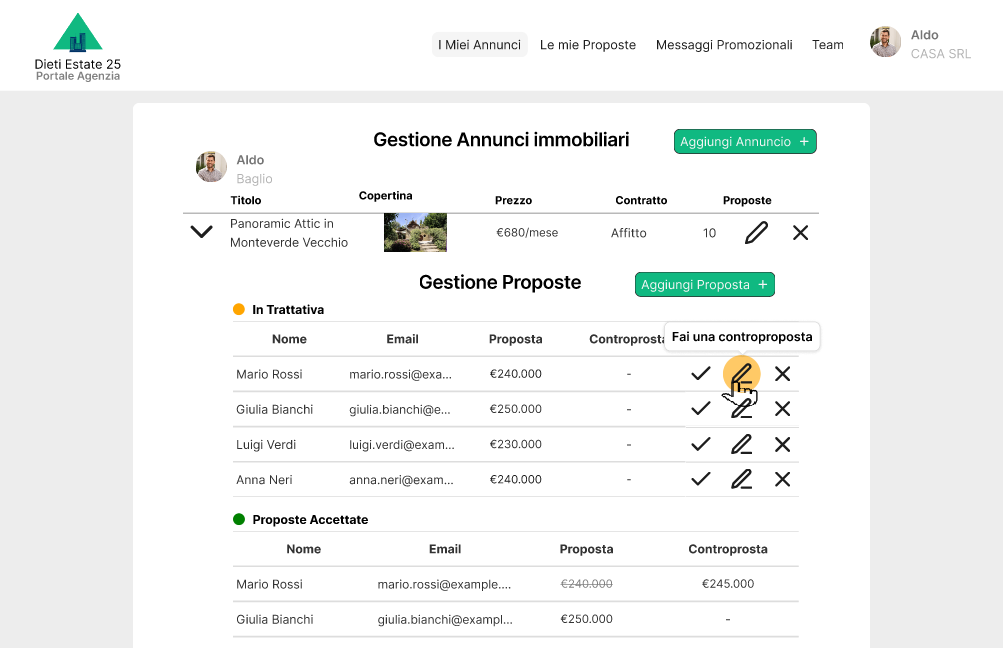
\includegraphics[width=0.7\textwidth]{Immagini/Mockup/controproposte/scenario principale/clickControproposta.png} \\
				Cockburn: step 1/2/3/4
			\end{tabular}
		};
		
		% Nodo per immagine 2 con didascalia sotto, posizionato a destra di img1
		\node (img2) [below=of img1] {
			\begin{tabular}{c}
				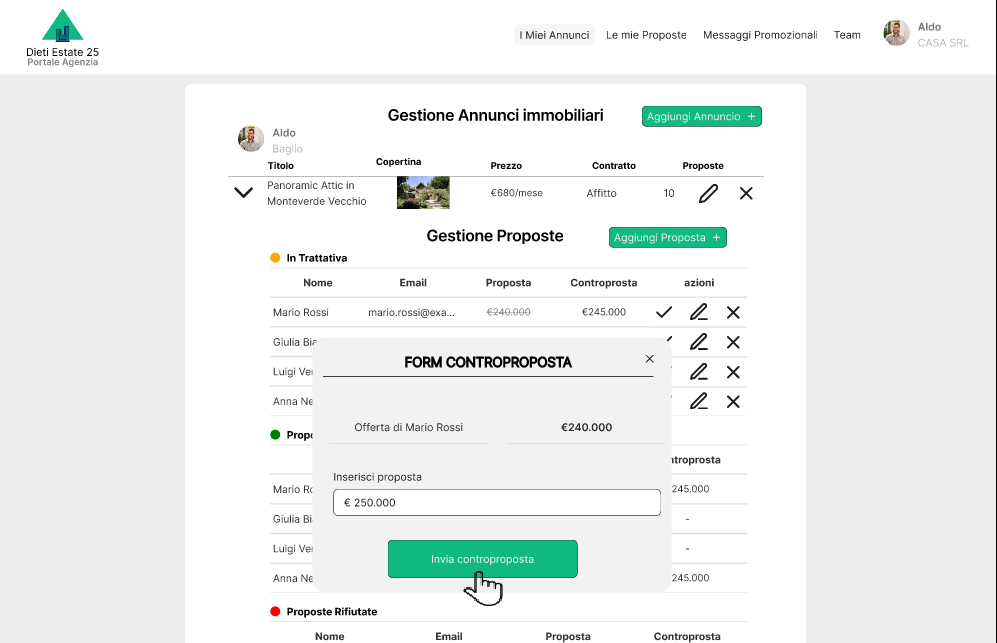
\includegraphics[width=0.7\textwidth]{Immagini/Mockup/controproposte/scenario principale/ClickInviaControproposta.png} \\
				Cockburn: step 5/6/7
			\end{tabular}
		};
		
		% Nodo per immagine 3 con didascalia sotto, posizionato sotto img2
		\node (img3) [below=of img2] {
			\begin{tabular}{c}
				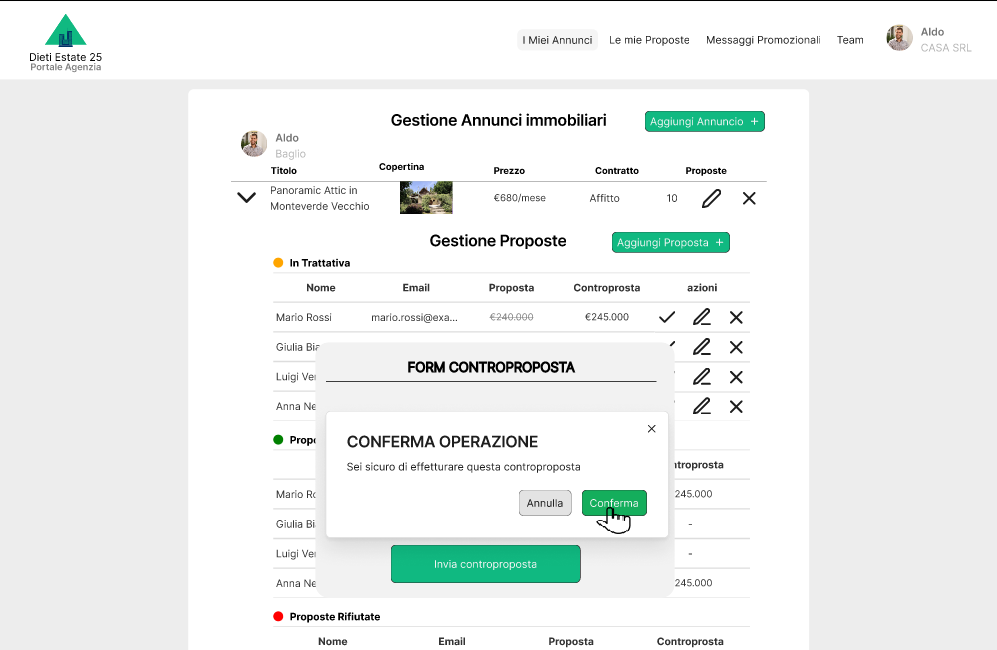
\includegraphics[width=0.7\textwidth]{Immagini/Mockup/controproposte/scenario principale/allertConfermaInvio.png} \\
				Cockburn: step 8/9/10
			\end{tabular}
		};
		
		% Disegna le frecce
		\draw[->, thick] (img1) -- (img2);
		\draw[->, thick] (img2) -- (img3);
		
	\end{tikzpicture}
	\caption{Mockup: scenario principale della tabella di Cockburn del caso d'uso: Fare una controproposta a un'offerta.}
	\label{fig:tikz_flow}
\end{figure}

\newpage

\begin{figure}[H]
	\centering
	\includegraphics[width=0.7\linewidth]{"Immagini/Mockup/controproposte/scenario principale/visualizzazioneControproposta"}
	\caption[Visualizzazione della controproposta]{}
	\label{fig:visualizzazionecontroproposta}
\end{figure}

\begin{figure}[H]
	\centering
	\begin{tikzpicture}[node distance=1.5cm and 1cm, auto]
		% Nodo per immagine 2 con didascalia sotto, posizionato a destra di img1
		\node (img1) {
			\begin{tabular}{c}
				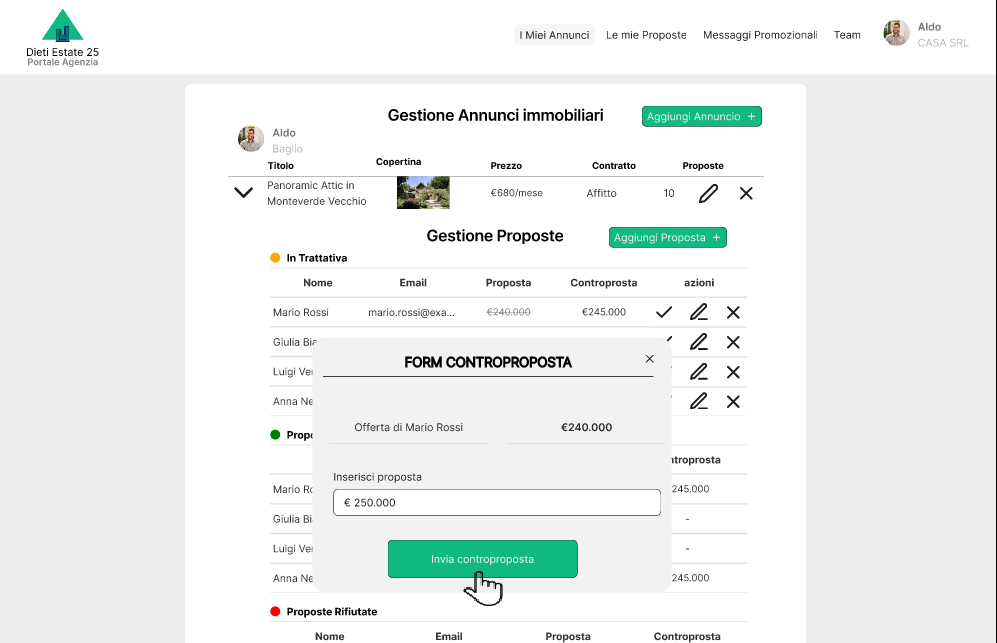
\includegraphics[width=0.7\textwidth]{Immagini/Mockup/controproposte/scenario principale/ClickInviaControproposta.png} \\
				Cockburn: step 6.A
			\end{tabular}
		};
		
		% Nodo per immagine 3 con didascalia sotto, posizionato sotto img2
		\node (img2) [below=of img1] {
			\begin{tabular}{c}
				\includegraphics[width=0.7\textwidth]{Immagini/Mockup/controproposte/Extensions A/MessaggioDiErrore.png} \\
				Cockburn: step 7.A
			\end{tabular}
		};
		
		% Disegna le frecce
		\draw[->, thick] (img1) -- (img2);
		
	\end{tikzpicture}
	\caption{Mockup: Extension A della tabella di Cockburn del caso d'uso: Fare una controproposta a un'offerta.}
	\label{fig:tikz_flow}
\end{figure}

\newpage




\newpage

\begin{figure}[H]
	\centering
	\begin{tikzpicture}[node distance=1.5cm and 1cm, auto]
		% Nodo per immagine 2 con didascalia sotto, posizionato a destra di img1
		\node (img1) {
			\begin{tabular}{c}
				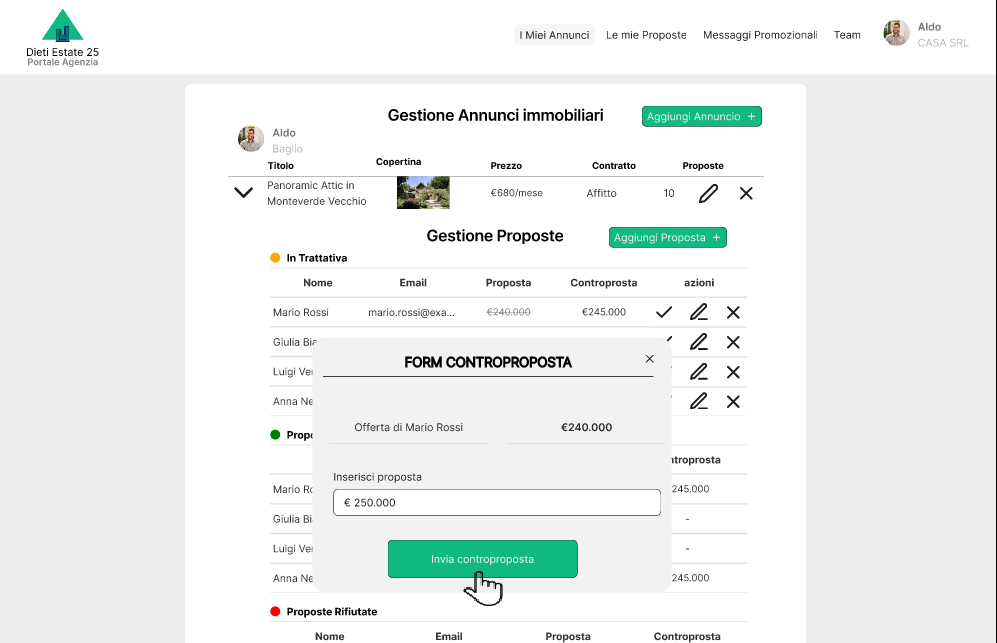
\includegraphics[width=0.7\textwidth]{Immagini/Mockup/controproposte/scenario principale/ClickInviaControproposta.png} \\
				Cockburn: step 7.B
			\end{tabular}
		};
		
		% Nodo per immagine 3 con didascalia sotto, posizionato sotto img2
		\node (img2) [below=of img1] {
			\begin{tabular}{c}
				\includegraphics[width=0.7\textwidth]{Immagini/Mockup/controproposte/Extensions B/MessaggioDiErrore.png} \\
				Cockburn: step 8.B
			\end{tabular}
		};
		
		% Disegna le frecce
		\draw[->, thick] (img1) -- (img2);
		
	\end{tikzpicture}
	\caption{Mockup: Extension B della tabella di Cockburn del caso d'uso: Fare una controproposta a un'offerta.}
	\label{fig:tikz_flow}
\end{figure}

\newpage




\newpage

subsubsection{Estensione C: Errore di Salvataggio della Controproposta}

In alcune circostanze, l’invio della controproposta può fallire a causa di problemi di connessione o di errori del server.  
Il sistema gestisce questa eventualità mostrando all’utente un chiaro feedback visivo sull’esito dell’operazione.

\subsubsection{Gestione dell’Errore e Comunicazione all’Utente}
Dopo aver cliccato su \textbf{“Invia controproposta”}, viene mostrato un breve stato di caricamento.  
Se il salvataggio non va a buon fine, compare un pop-up di allerta che informa l’agente dell’errore e della mancata registrazione della controproposta.

L’utente può chiudere l’allerta e tentare nuovamente l’operazione una volta ristabilita la connessione.  
Questo comportamento supporta la \textbf{recuperabilità dall’errore}, assicurando che l’utente non perda il lavoro svolto e possa riprovare senza dover reinserire tutti i dati.

\begin{figure}[H]
	\centering
	\begin{tikzpicture}[node distance=1.5cm and 1cm, auto]
		% Nodo per immagine 2 con didascalia sotto, posizionato a destra di img1
		\node (img1) {
			\begin{tabular}{c}
				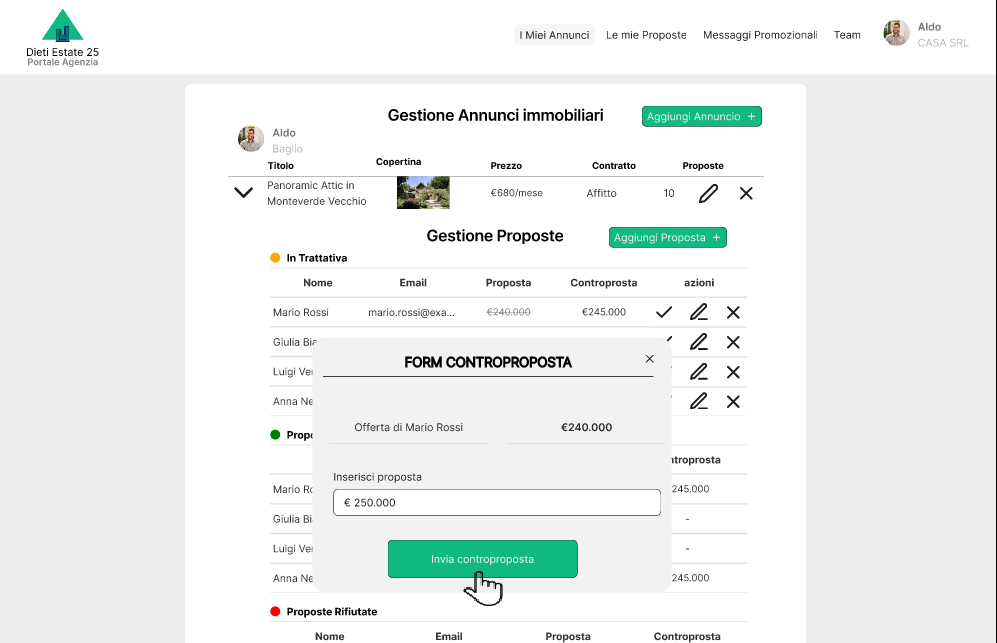
\includegraphics[width=0.7\textwidth]{Immagini/Mockup/controproposte/scenario principale/ClickInviaControproposta.png} \\
				Cockburn: step 7.C/8.C
			\end{tabular}
		};
		
		% Nodo per immagine 3 con didascalia sotto, posizionato sotto img2
		\node (img2) [below=of img1] {
			\begin{tabular}{c}
				\includegraphics[width=0.7\textwidth]{Immagini/Mockup/controproposte/Extensions C/MessaggioDiErrore.png} \\
				Cockburn: step 9.C
			\end{tabular}
		};
		
		% Disegna le frecce
		\draw[->, thick] (img1) -- (img2);
		
	\end{tikzpicture}
	\caption{Mockup: Extension C della tabella di Cockburn del caso d'uso: Fare una controproposta a un'offerta.}
	\label{fig:tikz_flow}
\end{figure}

\newpage


